\begin{frame}
 \frametitle{Main Questions}

What condition or conditions should

\begin{columns}[t]
  \column[T]{5cm}
  \begin{itemize}
    \item the position vector
    \item the coordinates
  \end{itemize}

of a point satisfy\\
for the point to be\\
on a specific\\

\begin{itemize}
    \item line $L$
    \item plane $\mathcal{P}$?
\end{itemize}
  \column[T]{7cm}
    \begin{figure}
        \psfrag{O}{$O$}
        \psfrag{x}{$x$}
        \psfrag{y}{$y$}
        \psfrag{z}{$z$}
        \psfrag{L}{$L$}
        \psfrag{Pi}{$\mathcal{P}$}
        \psfrag{P}{$P(x,y,z)$}
        \psfrag{Q}{$Q(x,y,z)$}
        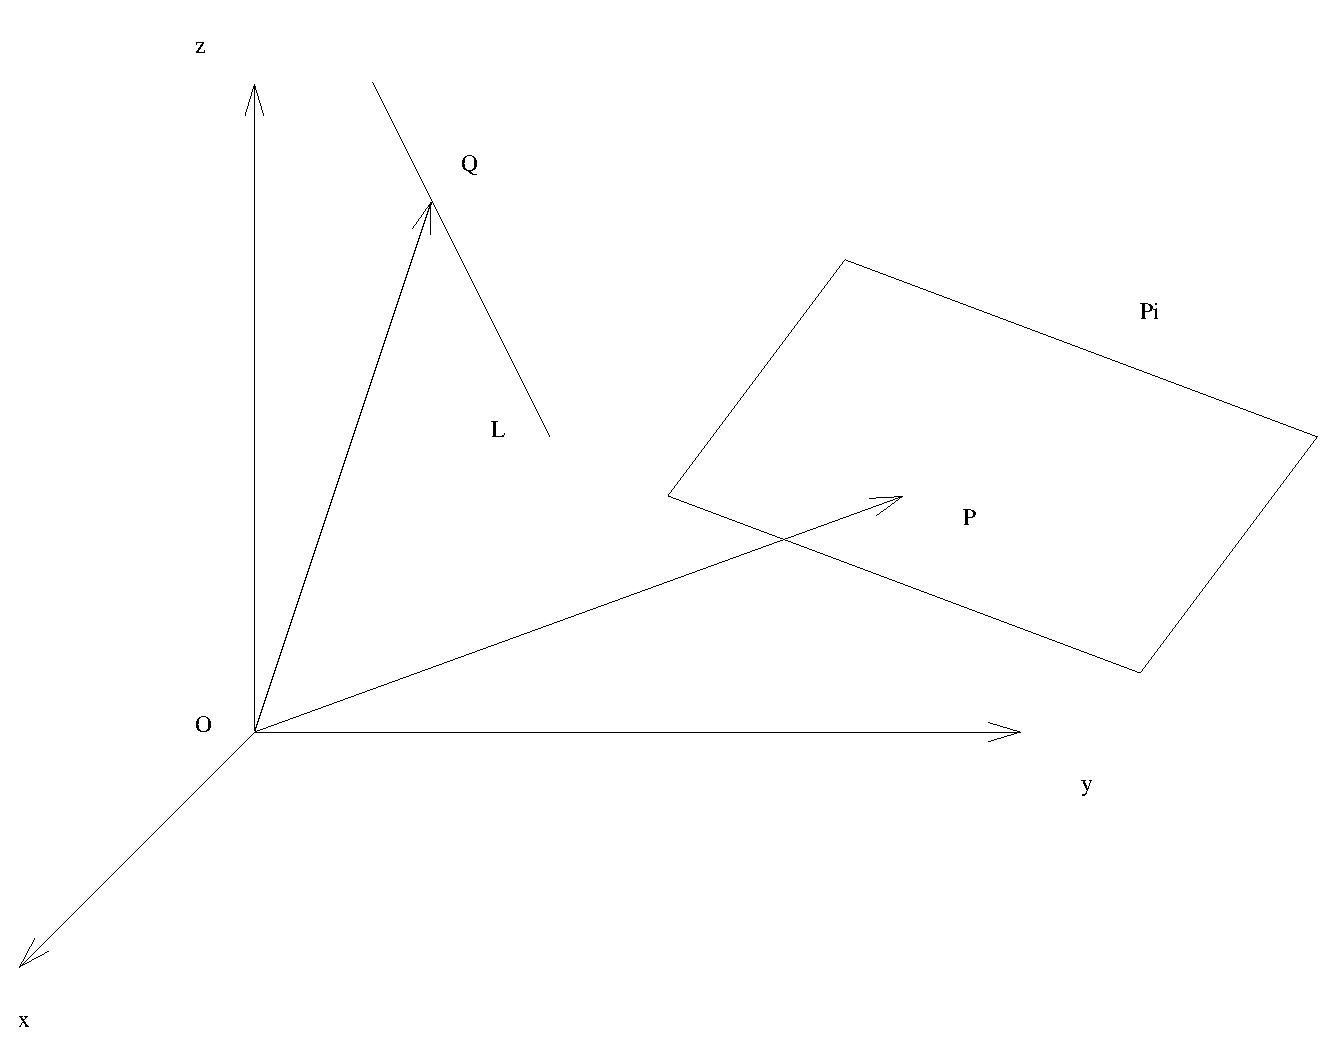
\includegraphics[height=2in]{../../modules/vectors/pictures/ok-lines_planes.eps}
    \end{figure}
\end{columns}

Condition(s) in terms of:
\begin{itemize}
    \item position vector $\Rightarrow$ vectorial equations;
    \item coordinates $\Rightarrow$ scalar equations.
\end{itemize}
\end{frame}